\secspace
\section{An Adaptive Mimicry Attack} 
\label{sec:eval-limitations}
In this section, we design, implement and evaluate an adaptive mimicry attack
designed to bypass the naive protection method described in
\S\ref{subsec:limitations}. 

It is made possible by the fundamental {\em temporal consistency} inherent to
all video content. Here, we propose {\em Perturbation Removal Attacks} (PRA)
that leverage temporal consistency to remove protective perturbations on
video frames, and present results measuring their efficacy using both
automated metrics and human feedback.

\secspace
\subsection{Perturbation Removal}

For naively protected video sequences, we develop an adaptive mimicry attack
that uses perturbation removal methods (PRM) to recover images that closely
approximate the original, unperturbed video frames. These are then used to
successfully train an image-based style mimicry model.  As such, for any
video sequence, a PRMs behaves like a frame extraction tool.

\para{``Combining'' consecutive frames.} PRMs remove protective perturbations
by combining multiple consecutive video frames (that share high visual
similarity) into a single frame. Intuitively, combining highly similar frames
will generally preserve the common pixel values inherited from the original
unprotected frames, while reducing or removing the pixel value changes made
by protective tools.  With this in mind, we consider three PRM approaches that
employ different ``combining'' functions across video frames.

\begin{packed_itemize}
\item \textbf{Selective Pixel Averaging} -- This approach generates a
  combined image out of consecutive frames, where each pixel is the average
  of the corresponding pixel values across the set of frames. This
  pixel-level ``averaging'' function ``smooths'' out the protective
  perturbations. Pixel averaging can be limited to more static regions and
  avoid pixels that capture motion across the frames. 
\item \textbf{FILM} -- Frame Interpolation for Large Motion
  (FILM)~\cite{reda2022film} is a neural network designed to generate
  temporally smooth videos from disjoint frames. We apply FILM to multiple
  perturbed frames from the same scene to reconstruct high quality images
  that closely resemble the original unperturbed frames, but don't retain
  perturbations from either input.
\item \textbf{Linear Interpolation} -- Linear interpolation is
  a technique for generating intermediate data points between a set of known
  points. Like the other approaches, pixel-level linear interpolation 
  across frames exploits lack of consistency between consecutive
  perturbations.
\end{packed_itemize}

\para{Implementing adaptive attacks.} We implemented 3 adaptive mimicry attacks, each
using one of the frame-aggregation approaches described above. In the rest of
this section, we present detailed results on all 3 adaptive attacks. The key
takeaway is that pixel averaging significantly outperforms the
alternatives. For brevity, we move implementation details of the other two
attacks to Appendix \ref{app:detailed-perturbation-removal}, and only provide
implementation details for the pixel averaging below. 

\begin{figure}[t]
  \centering
  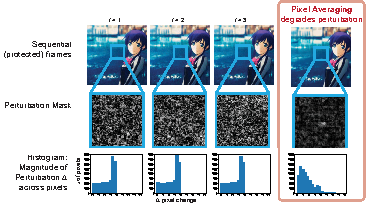
\includegraphics[width=1\columnwidth]{plots/pixel-averaging-scenario-04-eps-converted-to.pdf}
  \vspace{-0.2in}
  \caption{Averaging pixel values across highly similar consecutive frames
    successfully degrades the randomized protection pixel shifts across
    frames and largely restores the original unprotected frame. }
  \label{fig:pixel-averaging-attack}
\end{figure}

\emph{Pixel Averaging} approximates the original unprotected frame by
averaging pixels across highly similar consecutive frames (see
Figure~\ref{fig:pixel-averaging-attack}). Pixel level differences between
consecutive frames come from two sources: 1) natural changes between video
frames which we call \textit{movement}, and 2) differences in pixel changes
added by protective tools (\textit{perturbations}). Protective tools seek to
minimize visual impact, so the large majority of perturbation values are
constrained within a specific value. Thus an attacker can examine two
consecutive perturbed frames, and identify the source of each pixel
difference by filtering using a simple threshold ($\epsilon_p$). A well
chosen $\epsilon_p$ will separate pixel differences due to movement
($>\epsilon_p$) from pixel differences from protective tools
($<\epsilon_p$). The attacker measures pixel differences ($\Delta_p$) between
consecutive frames and only averages regions ($0 < \Delta_p <
\epsilon_p$). In practice, $\epsilon_p$ can easily be identified empirically
as a transition point between two levels of region sizes. In our tests, we
experimentally test pixel averaging across $n$ consecutive frames, and find
the best results around $n=5$.  We measure the quality of frames using CLIP
Aesthetic predictor~\cite{schuhmann2022laion} and perturbation removal using
metrics described in the following section. We show detailed results of the
tradeoff between perturbation removal vs. image quality in the appendix.

\subsection{Experimental Setup and Metrics}
To validate the efficacy of multiple perturbation removal methods, we add
naive protection to short scenes on an independent, per-frame basis. We then
test the adaptive mimicry attack by using each PRM to extract unprotected
frames from each video scenes. We compare different PRMs by measure the
amount of image level differences in the perturbations before vs. after our
attack using several automated metrics. We also measure end-to-end
success of the adaptive mimicry attack by training models on
extracted frames, and conducting a user study to gather human
feedback.

\para{Applying naive protection to all frames.}  We experiment on 5 diverse
datasets containing realistic videos of scenery and human actions, artistic
style videos, and video game style videos. We implement each of 3 protection
tools, Mist, Anti-DB, and Glaze.  For each scene, we identify and extract
scenes of highly similar frames, and apply ``naive protection'' by applying
each of 3 protection tools to each frame in selected frames. We apply each
PRM to the naively protected images to attempt to recover a good estimation
of the original images. We then compare original, naively protected, and
attacked naively protected images to each other.
As we show below, pixel-averaging significantly outperforms FILM and linear
interpolation in pixel level metrics.

\para{Performing style mimicry.} We perform style mimicry attacks under 3
``perturbation scenarios'': training mimicry models on 
clean (unperturbed) frames, frames protected by ``naive protection,'' and
frames extracted by adaptive attack following ``naive protection.''  Due to
high computation costs (multiple days per scene), we only compute end-end
results for the Pixel Averaging attack (shown to be strongest in pixel level
metrics above).
For each perturbation scenario, we chose ~30
scenes from a video, select (or extract) one image from each scene,
and train mimicry models on this set.  Further details on mimicry attack
configurations are in \S\ref{sec:eval}.

\para{Evaluation metrics.}  We evaluate the strength of perturbation removal
methods using pixel level metrics (Mean Pixel Difference and Latent $L_2$ Norm). 
We evaluate end-to-end results on style mimicry using human feedback
(User Study). We briefly describe these metrics below, and give more details later in
\S\ref{sec:eval}.

\begin{packed_itemize}
\item{\em Latent $L_2$ Norm.} We employ the image encoder used in diffusion models
  to calculate image representations of perturbed and non-perturbed (original)
  frames, and then calculate the $L_2$ distance between them as a measure
  of proximity between two images. Thus, a successful perturbation removal
  would minimize the latent $L_2$ norm, while a robust system should maintain a
  high latent $L_2$ norm.

\item{\em Mean Pixel-Difference.}  We measure differences between images at a
  pixel level, motivated by the $l_{inf}$ bounded pixel changes that all
  protection tools (Mist, Anti-DB, Glaze) use to limit visual artifacts. We
  define Mean Pixel Difference (MPD) as the average of all pixel differences
  between a perturbed image and clean image. Similar to the latent $L_2$ norm, 
  a higher MPD signals higher protection.

\item{\em Human feedback.}  We perform a user study to evaluate the success
  of adaptive mimicry attacks, by asking participants to look at images
  produced by a mimicry model, and compare it to original video frames.  We
  ask participants to rate the success on a 5-level Likert scale (ranging
  from ``not successful at all'' to ``very successful''). Following existing
  work, we define protection success rate (PSR) as the percent of
  participants who rated the style mimicry as ``not very successful'' or
  ``Not successful at all.''
\end{packed_itemize}

\begin{figure}[t]
  \centering
  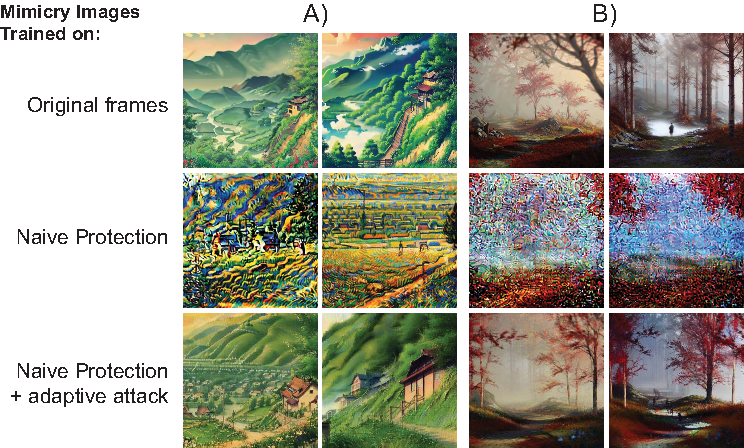
\includegraphics[width=1\columnwidth]{plots/pixel-avging-success-eps-converted-to.pdf}
  \vspace{-0.3in}
  \caption{Visual examples of adaptive mimicry attack. Three rows of
      mimicry images generated by models trained on 1) original video frames,
    2) video frames protected naively, and 3) video frames recovered after
    perturbation removal using pixel averaging.}
  \label{fig:style-mimicry-attacked}
\end{figure}

\begin{table}[t]
  \centering
    \resizebox{0.5\textwidth}{!}{
    \centering
\begin{tabular}{c|cccc}
 Protection Tool  & Protected          & Pixel Avg                   & FILM Interpolation & Linear Interpolation \\ \hline
  Glaze          & 390.05 $\pm$ 25.17 & \textbf{295.55 $\pm$ 52.02} & 391.51 $\pm$ 62.86 & 355.58 $\pm$ 44.38   \\
  Mist           & 474.87 $\pm$ 42.14 & \textbf{334.62 $\pm$ 56.72} & 437.78 $\pm$ 64.89 & 411.27 $\pm$ 51.89   \\
  Anti-DB        & 405.17 $\pm$ 37.55 & \textbf{283.41 $\pm$ 58.99} & 378.43 $\pm$ 67.34 & 352.10 $\pm$ 52.30  
  \end{tabular}
  }\caption{Latent $L_2$ Norm between original frames, protected frames
    and protected frames after perturbation removal.}
\label{tab:loss-removal-results}
\vspace{-0.2in}
\end{table}


\begin{table}[t]
  \centering
    \resizebox{0.5\textwidth}{!}{
    \centering
\begin{tabular}{c|cccc}
  Protection Tool & Protected          & Pixel Avg                   & FILM Interpolation & Linear Interpolation \\ \hline
  Glaze          & 111.30 $\pm$ 12.94 & \textbf{90.04 $\pm$ 14.13}  & 97.83 $\pm$ 13.73  & 96.16 $\pm$ 14.47    \\
  Mist           & 121.25 $\pm$ 9.48  & \textbf{107.10 $\pm$ 16.33} & 112.99 $\pm$ 14.36 & 113.03 $\pm$ 15.46   \\
  Anti-DB        & 124.86 $\pm$ 8.93  & \textbf{103.75 $\pm$ 17.70} & 110.29 $\pm$ 15.52 & 110.39 $\pm$ 16.42  
  \end{tabular}
  }\caption{Mean Pixel Difference between original frames, protected frames,
    protected frames after perturbation removal.}
\label{tab:pd-removal-results}
\vspace{-0.2in}
\end{table}


\subsection{Adaptive Mimicry Results}

Next we present results of our experiments on the adaptive attack.

\para{Similarity of recovered frames to original frames.} We compare
{\em latent $L_2$ norm} 
between the original frames, the protected frames, and protected frames after
protection removal.  Table~\ref{tab:loss-removal-results} shows FILM to
have minimal impact, and that Pixel averaging does the best to minimize loss
for the recovered frame, suggesting that it is closer to the original frame
in the feature space.

We also compare {\em mean pixel differences} between the original
frames, protected frames, and protected frames after protection removal.
Table~\ref{tab:pd-removal-results} shows that again, pixel averaging method
outperforms against all protection tools, and minimizes the pixel differences
between the extracted frame and the original. 

\para{Style mimicry attack on recovered images.}  Finally, we use a user
study to evaluate the end-to-end success of the adaptive mimicry attack using
pixel-averaging to overcome a per-frame application of protection tools.
Table~\ref{tab:user-study-removal-results} shows that users agree, the
adaptive mimicry attack with pixel averaging basically produces mimicry
results similar to mimicry on original unprotected video frames (PSR baseline
value of 17.65 for unprotected video frames).
Figure~\ref{fig:style-mimicry-attacked} shows samples of mimicry images from
models trained on original frames, protected frames, and protected frames
under adaptive attack. Clearly the adaptive attack is able to bypass
protection and restore mimicry success.

These results validate our concerns, that a naive, frame by frame application
of protection tools to videos is insufficient to prevent image mimicry. We
need to extend these anti-mimicry tools to restore their protection in the
video domain.